\mychapter{Fundamentação Teórica}{cap:fundamentacao}

Para que se obtenha um melhor entendimento acerca do tema proposto, neste  capítulo  serão  apresentadas  as  fundamentações  teóricas, obtidas por meio da realização da revisão bibliográfica dos conceitos e técnicas presentes no estado da arte.

\section{Representação do espaço de probabilidade}

A transformação de uma série temporal em uma distribuição de probabilidade (PDF) $P$ permite avaliar o conteúdo informacional acerca da dinâmica do sistema e dos processos subjacentes, descrevendo-os de forma mensurável e observável~\citep{entropyAndInformationTheory}.
Através desta caracterização é possível utilizar de métricas do espaço PDF, permitindo comparar diferentes conjuntos e classificá-los de acordo com as propriedades dos processos subjacentes. 
Podemos assim, por exemplo, classificar uma série entre estocástica ou determinística.

A ideia das técnicas não paramétricas consiste em construir o histograma de algum atributo da série temporal, e extrair dele métricas de Teoria da Informação.
Os atributos são os mais variados~\citep{Kowalski2011DistancesIP}, dentre eles: 
\begin{enumerate}[label=(\alph*)]
\item Padrões ordinais~\citep{ROSSO2},
\item Histogramas~\citep{article3,DEMICCO20083373},
\item Dinâmica simbólica binária~\citep{PhysRevLett},
\item Análise de Fourier~\citep{article}, e 
\item Transformada wavelet~\citep{ROSSO3}. 
\end{enumerate}

Todas estas metodologias são capazes de capturar aspectos globais de dinâmicas complexas. 
No entanto, não é trivial encontrar uma representação simbólica significativa da série original. 
Assim, por considerar a causalidade temporal dos dados, a abordagem de~\citet{article2} revela detalhes importantes da estrutura ordinal da série temporal.

\section{Método de simbolização de Bandt e Pompe }

De acordo com a abordagem de Bandt e Pompe, substituímos a série por sequências de postos, obtidos pela análise desta ao longo do tempo.

Dada uma série temporal a tempo discreto $X = {x_t:1\leq t\leq M}$, uma dimensão $D$ e um tempo de atraso (delay) $\tau$, o particionamento é efetuado por meio da reorganização do sistema em conjuntos seguindo os seguintes passos:
\begin{description}
\item[Composição dos grupos:] A série inicialmente será particionada em conjuntos de tamanho $D$ e delay $\tau$, possuindo a seguinte estrutura: 
		 $$(s) \mapsto (X_{\tau+1},\ldots, X_{\tau+D}).$$  

\item[Formação dos padrões:] Cada grupo formado anteriormente é então relacionado a um padrão ordinal $\pi$ de ordem $D$, como se observa abaixo:
		$$ \{1, 2,\ldots, D-1, D\}. $$

\item[Elaboração dos símbolos:] É realizada então a permutação dos elementos dos grupos, de tal forma que estes estejam ordenados de forma crescente.
		$$ x_{t+1} \leq x_{t} \leq ... \leq x_{D-1} \leq x_{D}. $$ 
\end{description}

De mesmo modo é impreterível que a permutação ocorra com os elementos dos padrões relacionados a cada grupo, pois estes corresponderam aos símbolos da série.

\begin{figure}[!ht]
	\begin{center}
		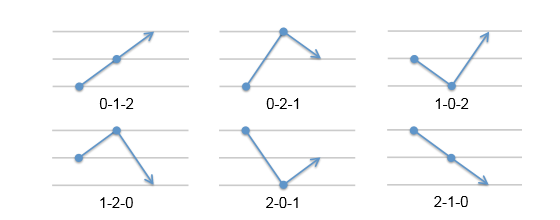
\includegraphics[width=0.7\columnwidth]{imagens/padroes.png}
        \caption{Representação gráfica dos padrões com dimensão $D=3$.}
	\end{center}
\end{figure}

A literatura apresenta duas maneiras de definir o mapeamento de padrões~\citep{tiedvalues}:  

\begin{enumerate}[label=(\alph*)]
\item Ordenando as posições dos grupos em ordem cronológica (Permutação de Classificação), e 
\item Ordenando os índices de tempo de acordo fileiras dos elementos do subconjunto (Permutação do Índice Cronológico).
\end{enumerate}

Logo abaixo, podemos analisar como se comporta a representação gráfica dos padrões ordinais através de cada um desses mapeamentos.

\begin{figure}[!ht]
	\begin{center}
		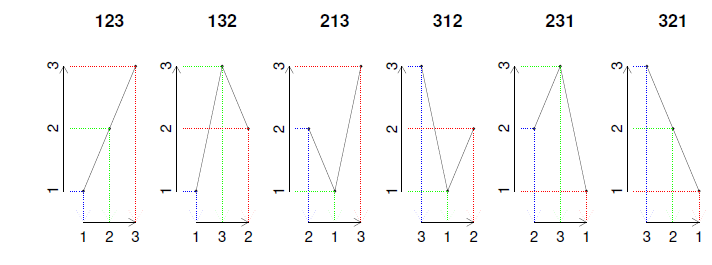
\includegraphics[width=0.7\columnwidth]{imagens/rankPermutation.png}
        \caption{Mapeamento por Permutação de Classificação~\citep{tiedvalues}}
	\end{center}
\end{figure}

\begin{figure}[!ht]
	\begin{center}
		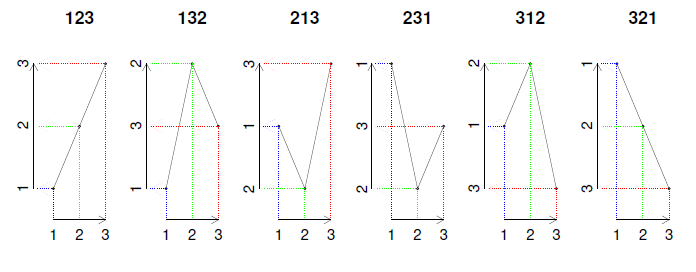
\includegraphics[width=0.7\columnwidth]{imagens/chronologicalIndex.png}
        \caption{Mapeamento por Permutação do Índice Cronológico~\citep{tiedvalues}}
	\end{center}
\end{figure}
				
%=========================================================

\section{Distribuição de probabilidade de Bandt e Pompe}

Em estatística, uma distribuição discreta de probabilidade refere-se à distribuição de frequências relativas para os resultados de um espaço amostral, apontando a quantidade de vezes em que um determinado elemento do conjunto assume cada um dos seus possíveis valores.

Logo:
 $$\sum_{n}^{i=1} Pi = 1. $$ 

Assim, a distribuição de probabilidade de Bandt \& Pompe consiste no cálculo da distribuição dos símbolos da série diante das $D!$ possíveis permutações dos padrões ordinais $\pi$ de comprimento $D$.

%Desse modo, tal propriedade é vista através da seguinte fórmula:
%$$p(\pi)=\frac{\left \{\#t | 0 \leq t \leq M - D + 1, (x_{t+1}, \ldots, x_{t+D}) \indent do \indent tipo \indent \pi\right \}}{M-D+1}  $$ 

Uma grande vantagem de sua utilização refere-se ao fato da distribuição de probabilidade tornar-se invariante com respeito às transformações monótonas, propriedade extremamente desejada na análise das séries.

Uma vez calculado o histograma de padrões $\bm p=(p_1,\dots,p_{D!})$, isto é, a função de probabilidade, o próximo passo será obter descritores.

\section{Entropia de permutação}

A Entropia mede o desordem ou a imprevisibilidade de um sistema caracterizado por uma função de probabilidade $\bm p$.
Neste trabalho, citaremos três modelos de entropia: de Shannon, de Tsallis e de Rényi.

Proposta em 1948, a entropia de Shannon consiste de uma variação da Entropia de Boltzmann-Gibbs~\cite{shannon}.
Ela é definida por $H(\bm p) = -\sum_{i}^{D} p_i \log p_i $.
Os seus valores mínimo ($0$) e máximo ($1$) ocorrem para os casos em que um único evento tem probabilidade $1$, e para eventos equiprováveis, respectivamente, isto é, para a certeza e a incerteza completas. 

Tsallis propôs um novo modelo~\cite{entropyInformation}, ampliando o  conjunto de aplicações abordado por Boltzmann:
$H_a(\bm p) ={(a-1)}^{-1}(1 - \log \sum_{i=1}^{D!}p_i^a)$, com $a \neq 1$.

A entropia de Rényi é uma generalização da entropia de Shannon, sendo aplicada em Teoria da Informação como um índice estatístico de diversidade ou aleatoriedade~\cite{Tsallis1988}: $H_a(\bm p) ={(1-a)^{-1}}\log \sum_{i=1}^{D!}p_i^a$.


\section{Distância Estocástica}

A habilidade da entropia de capturar propriedades do sistema é limitada, logo se faz necessário a utilização da mesma em conjunto de outros descritores, para assim realizar uma análise mais completa.
Outras medidas interessantes são distâncias entre a função de probabilidade $\bm h$ e uma medida de probabilidade que descreva um processo não informativo, tipicamente a distribuição uniforme.

Para mensurar a similaridade entre duas distribuições de séries temporais, todas as funções que calculam determinada característica devem respeitar algumas propriedades. 

Sendo $c1, c2$ e $c3$ objetos do universo de objetos, devem ser mantidas as seguintes particularidades:

\begin{itemize}

	\item Simetria:
	$D(c1,c2) = D(c2,c1)$
	\item Similaridade:
	$D(c1,c1) = 0$
	\item Positividade:
	$D(c1,c2) = 0$ se, e somente se, $c1 = c2$
	\item Desigualdade triangular:
	$D(c1,c3) \leq D(c1,c2) + D(c2,c3)$

\end{itemize}

Também consideradas no estudo relatado, as chamadas divergências são aquelas na qual seguem apenas duas das particularidades acima, positividade e similaridade.

\begin{figure}[!hbt]
	\begin{center}
		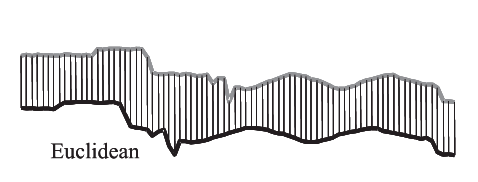
\includegraphics[width=0.7\columnwidth]{imagens/distance.png}
        \caption{Representação da Distância Euclidiana}
	\end{center}
\end{figure}

A Tabela~\ref{Tab:Distancias} mostra algumas possíveis medidas de distância $d(\bm p,\bm q)$ entre duas funções de probabilidade $\bm p=(p_1,\dots)$ e $\bm q=(q_1,\dots)$, definidas sobre o mesmo suporte.

\begin{table}[hbt]
\caption{Distâncias Estocásticas}\label{Tab:Distancias}
\centering
\begin{tabular}{lc}\toprule
Euclidiana					& $ \sqrt{\sum_i(q_i-p_i)^{2}}$\\
Manhattan					& $ \sum_{i}|q_i-p_i|$\\
Chebyshev					& $ \max_i\{|q_i-p_i|\}$\\
Kullback-Leibler			& $ \sum_{i}q_i \log\frac{q_i}{p_i}$\\
Jensen-Shannon				& $ \sum_{i} \Big(p_i \log\frac{p_i}{q_i} + q_i \log\frac{q_i}{p_i}\Big)$\\
Wotters						& $ \cos^{-1}\sum_{i} \sqrt{p_i q_i}$ \\
Bhattacharya				& $ -\log\sum_{i}\sqrt{p_i q_i}$ \\
\bottomrule
\end{tabular}
\end{table}

Outras distâncias e relações entre elas podem ser vistas no livro de Deza e Deza~\citep{EncyclopediaofDistances}.

\section{Complexidade Estatística}

Por definição complexidade refere-se a um conjunto de coisas ligadas por um nexo comum. Inversamente a entropia, a complexidade estatística procura encontrar estruturas de interação e dependência entre os elementos de uma dada série, tratando-se de um fator extremamente importante no estudo de sistemas dinâmicos.

Essa propriedade é definida por meio da fórmula desenvolvida por Lopèz-Ruiz, Mancini e Calbet, onde uma Entropia e uma Distância podem ser combinadas no atributo Complexidade Estatística: $C(\bm h, \bm p) = H(\bm h)d(\bm h, \bm p)$ para aumentar o seu poder de descrição~\citep{article5,FELDMAN1998244,LOPEZRUIZ1995321}:
Uma escolha conveniente é a complexidade de Jensen-Shannon, dada por
 \begin{equation}
 C_{\text{JS}}(\bm h) = H_{\text{S}}(\bm h) . Q_{\text{JS}}(\bm h, \bm p),
 \end{equation}
em que $H_{\text{S}}$ é a entropia de Shannon normalizada, $\bm h$ a função de probabilidade da série, $\bm p$ a distribuição uniforme e $Q_{\text{JS}}$ é a distância de Jensen-Shannon.

\section{Plano HC}

 O plano de entropia complexidade refere-se ao gráfico bidimensional entre a Entropia normalizada $H(p)$ (eixo horizontal) versus a Complexidade Estatística $Clmc$ (eixo vertical). 

 Por intermédio de tal ferramenta se faz possível descobrir a natureza da série, determinando se esta trata de uma sequência caótica, estocástica ou determinística, analisando o seu comportamento, visto que estes possuem diferentes dinâmicas. De acordo com a segunda lei da termodinâmica:
 \begin{quote}
A quantidade de entropia de qualquer sistema isolado termodinamicamente tende a incrementar-se com o tempo, até alcançar um valor máximo. 
 \end{quote}

 Logo, como a entropia varia uniformemente com o tempo, podemos concluir que o plano Complexidade-Entropia além de analisar a interação entre estas duas características, também verifica a evolução temporal de $Clmc$.

 O plano Entropia-Complexidade também é conhecido como “O plano de causalidade entre a entropia e a complexidade”, tendo em vista que no ramo da estatística causalidade refere-se a relação entre as causas dos fenômenos e seus respectivos efeitos e resultados. Assim podemos inferir que como a própria nomenclatura sugere, o diagrama relaciona os dados resultantes do cálculo da entropia e da complexidade estatística e as suas características estimadas pela teoria da informação. 

\begin{figure}[!hbt]
	\begin{center}
		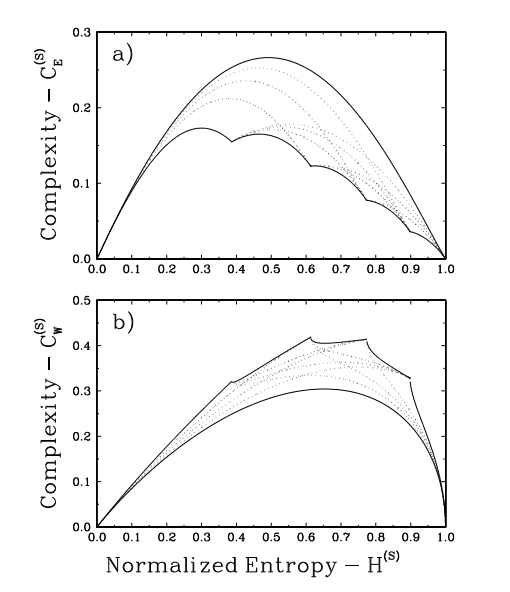
\includegraphics[width=0.6\columnwidth]{imagens/graficoComplexidade.png}
        \caption{Gráficos Complexidade-Entropia em relação à entropia de Shannon e as distâncias Euclidiana e de Wootters.}
	\end{center}
\end{figure}
 
Cada série temporal $\bm x$ pode, então, ser mapeada no ponto $(H_{\text{S}}, C_{\text{JS}})$.
O conjunto de todos os pontos possíveis forma o \textit{mapa Entropia-Complexidade}, e a posição do ponto nesse plano é um descritor das propriedades da dinâmica subjacente à série~\cite{OrdinalPatternProbabilities}.
A forma desse plano depende do comprimento $D$ dos padrões~\cite{MARTIN2006439}.
